\documentclass[10pt]{article}
\usepackage{../be-my-concrete}
\usepackage{../be-my-geometry}
\usepackage{../extra-topology}

\begin{document}
\dz{8}
\date{7 февраля 2025}


\tableofcontents


\begin{tasks}
    \addcontentsline{toc}{section}{Задача 1}\item Верно ли, что компактное подмножество произвольного то\-по\-ло\-ги\-чес\-ко\-го пространства обязательно является замкнутым? Докажите или приведите контрпример.
    \begin{proof}
        [Решение]
        Приведу два контрпримера.
        
        \textsc{Пример 1.} Пусть $X$ -- произвольное непустое множество, тогда $$\T = \{X, \emptyset\}.$$
        Пусть $A \subsetneq X$, тогда $X\setminus A \not \in \T.$ Значит $A$ не замкнуто. Из любого его покрытия можно выделить конечное подпокрытие -- это просто множество $X$.

        \textsc{Пример 2.} Рассмотрим $\mathbb F_2 \coloneq \{0,1\}$, введём на нём топологию: \[\T = \{\emptyset, \{0\}, \{0,1\}\}.\]
        
        Тогда рассмотрим $\{0\} \subset \mathbb F_2$. $$\mathbb F_2 \setminus \{0\} = \{1\} \not\in \T.$$ Значит $\{0\}$ не замкнуто. Из любого открытого покрытия можно выделить конечное подпокрытие -- или множество $\{0\}$, или всё $\mathbb F_2.$
        
        \ans{Нет.}
    \end{proof}
    
    \addcontentsline{toc}{section}{Задача 2}\item Фундаментальная последовательность (в метрическом пространстве) имеет сходящуюся подпоследовательность тогда и только тогда, когда и вся последовательность сходится. Докажите.

    \begin{proof}
        [Решение]
        
        Пусть $(x_n)_{n\in\N}$ фундаментальная последовательность, а $(x_{n_k})_{k\in \N}$ сходится к $A$. Тогда 
        \begin{equation}
            \begin{aligned}
                &(\forall \epsilon > 0)(\exists N \in \N)(\forall n > N)(\exists p \in \N)\quad \begin{cases}
                    \rho(x_n, x_{n+p}\footnotemark) < \rfrac \epsilon 2 \\
                    \rho(x_{n+p},A) < \rfrac \epsilon 2
                \end{cases} \implies \\
                &\implies \rho(x_n, A) \leqslant \rho(x_n, x_{n+p}) + \rho(x_{n+p}, A) \leqslant 2 \cdot \frac \epsilon 2 = \epsilon.
            \end{aligned}
        \end{equation}
        \footnotetext{Здесь $x_{n+p}$ выбрано так, чтобы $x_{n+p}$ было частью подпоследовательности $(x_{n_k})_{k\in \N}$.}
        
        Пусть фундаментальная последовательность $(x_n)_{n\in\N}$ сходится. Тогда и подпоследовательность равная самой последовательности $(x_n)_{n\in\N}$ сходится.
    \end{proof}
    %\pagebreak

    \addcontentsline{toc}{section}{Задача 3}\item Рассмотрим карту Москвы. Положим на нее такую же карту, но меньшего масштаба, причем будем считать, что маленькая карта целиком помещается на большой карте. Докажите, что можно так проколоть обе карты тонкой булавкой, чтобы на обеих картах точка прокола соответствовала одной и той же точке Москвы.
    \begin{figure}[ht]
        \centering
        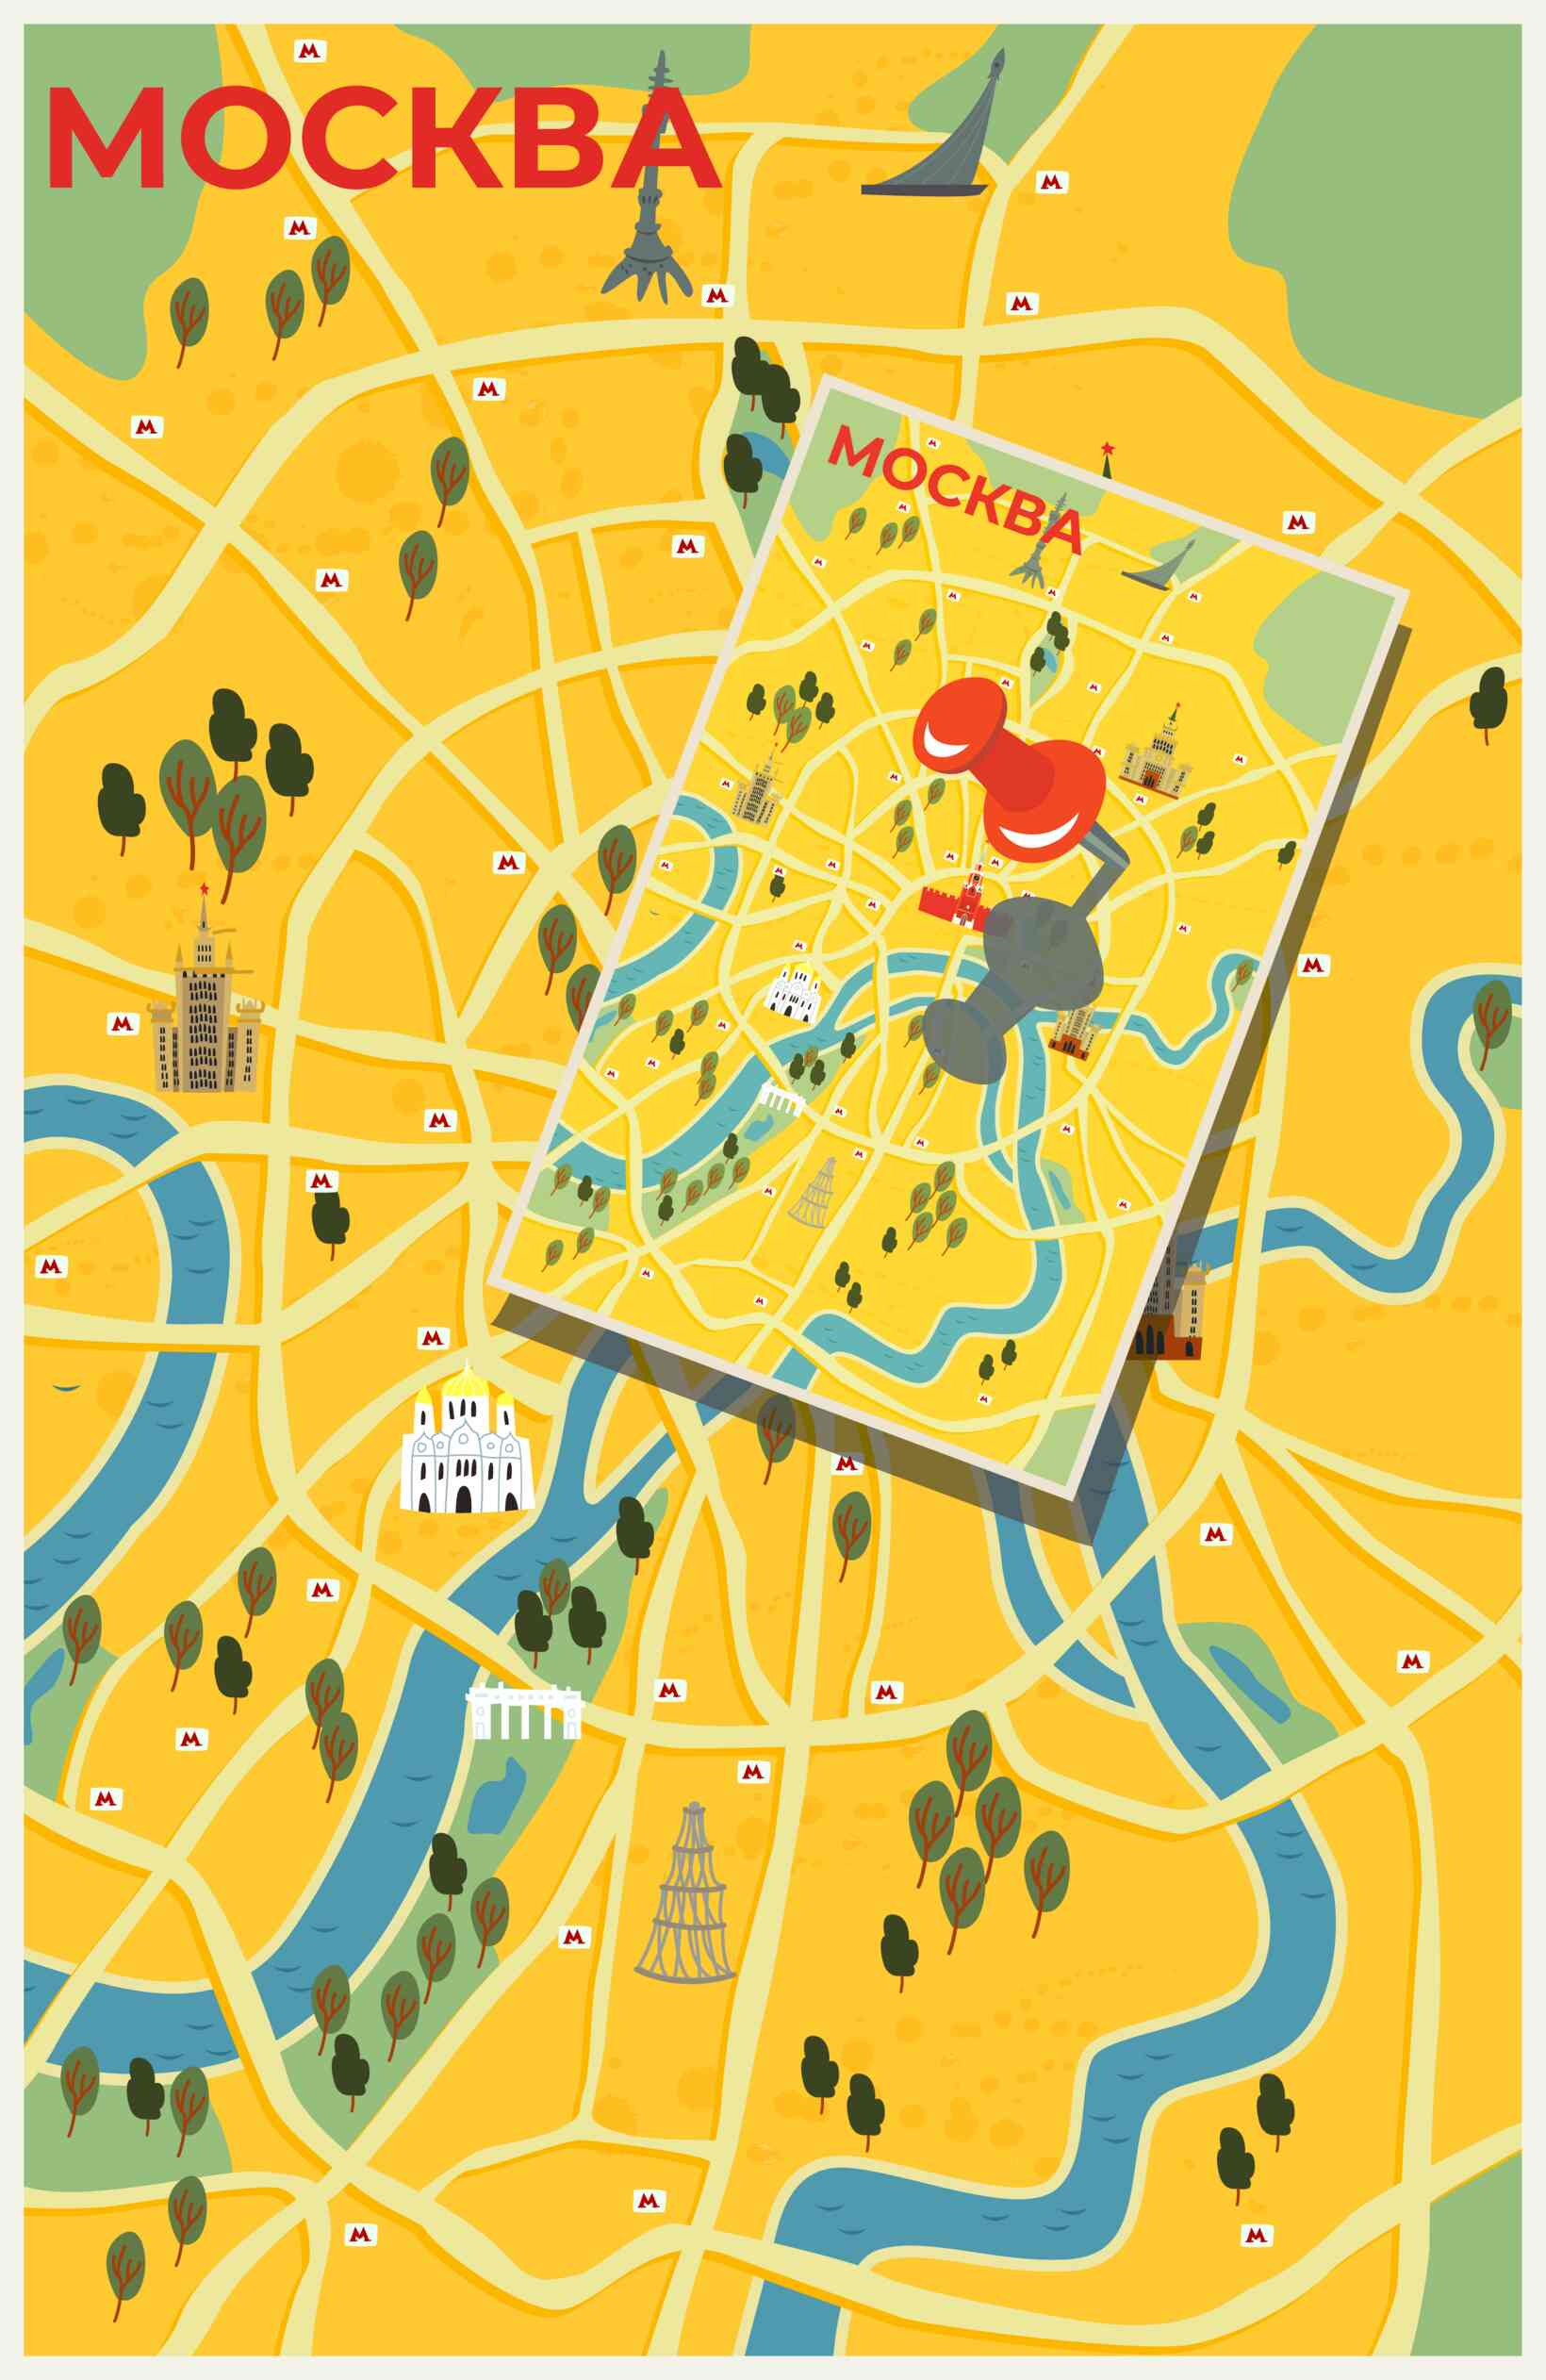
\includegraphics[width=0.5\linewidth]{../graphics/карта мск_Монтажная область 1.jpg}
    \end{figure}

    \begin{proof}
        [Решение]
        Наши карты является компактными подмножествами $\R^2$, обозначим через $M$ нашу изначальную карту. Существует сжимающее отображение $f\colon M \to M$, которое состоит из композиции гомотетии $H_k$ с коэффициентом $k < 1$ и осевых симметрий $(\ell_\lambda)_{\lambda\in\Lambda}$\footnote{Конечно же, можно сказать, что таких отражений не больше двух, но это несущественно.}

        Выберем произвольную точку $x_0 \in M$ и определим $x_1 \coloneq f(x_0)$, следующие точки определяются аналогично. 
        \begin{equation}
            \rho(x_{n+1}, x_n) = k\cdot\rho(x_n, x_{n-1}) = k^n\rho(x_1, x_0).
        \end{equation}
        Тогда последовательность $(x_n)_{n\in \N}$ фундаментальная: \begin{equation}\begin{aligned}
            \rho(x_n, x_m) \leqslant \rho(x_n, x_{n-1}) + \ldots + \rho(x_{m+1}, x_m)  \leqslant \\ \leqslant \rho(x_1, x_0)(q^{n-1} + \ldots + q^m) \leqslant \rho(x_1, x_0)\frac{q^m}{1-q}
        \end{aligned}
        \end{equation}
        Тогда в силу полноты $\R^2$ существует предел \begin{equation}
            x^\star \coloneq \lim_{n\to\infty}x_n = \lim_{n\to \infty} T(x_{n-1}) =T\left(\lim_{n\to \infty}x_{n-1}\right) = T(x^\star).
        \end{equation} 
        Точка $x^\star$ -- искомая.
    \end{proof}

    \addcontentsline{toc}{section}{Задача 4}\item Пусть $X$ -- метрическое пространство, точками которого являются последовательности действительных чисел $x_1,x_2,\ldots, x_n,\ldots$, такие, что $|x_n|\leqslant \rfrac 1 n$ для всех $n$, а метрика определяется формулой \[\rho(x,y)^2=\sum_{n=1}^\infty (x_n-y_n)^2.\] Здесь $x_n$, $y_n$ -- это члены последовательностей $x$, $y$ (соответственно) с номером $n$. Проверьте, что это действительно метрика. Докажите, что пространство $X$ является полным и вполне ограниченным, а следовательно, компактным. Для всякого $\epsilon>0$ оцените сверху минимальное количество точек в $\epsilon$-сети пространства $X$.
    \pagebreak
    \begin{proof}
        [Решение]
        Проверим, что это метрика. Аксиомы \emph{тождества} и \emph{симметричности} очевидны. Осталось проверить лишь \emph{неравенство треугольника.}
        \begin{DispWithArrows}[displaystyle, wrap-lines, tagged-lines = 4, mathindent = 0 pt]
            &(\rho(x,y)+\rho(z,x))^2 = \rho(x, y)^2 + \rho(z,x)^2 + 2\rho(x,y)\rho(z,x) = \\
            &= \sum_{n=1}^\infty (x_n-y_n)^2 + \sum_{n=1}^\infty(z_n-x_n)^2 + 2\sqrt{\sum_{n=1}^\infty (x_n-y_n)^2}\sqrt{\sum_{n=1}^\infty(z_n-x_n)^2} \geqslant \Arrow[down]{Неравенство КБШ} \\ 
            &\geqslant \sum_{n=1}^\infty (x_n-y_n)^2 + \sum_{n=1}^\infty(z_n-x_n)^2 + 2\sum_{n=1}^\infty (x_n-y_n)(z_n-x_n) = \\ &= \sum_{n=1}^\infty\left((x_n-y_n)^2 + (z_n-y_n)^2+2(x_n-y_n)(z_n-x_n)\right) = \\ &= \sum_{n=1}^\infty (x_n-y_n+z_n-x_n)^2 = \rho(z, y)^2. 
        \end{DispWithArrows}
        \begin{remark}
            Нужно сказать, почему мы можем использовать \emph{неравенство Коши-Буняковского-Шварца}, ведь оно верно лишь для конечных сумм. Оно верно и в этом случае, так как наши ряды: $\sum_{n=1}^\infty (x_n-y_n)^2$ и $\sum_{n=1}^\infty (z_n-x_n)^2$ сходятся\footnote{Пропускаю тривиальное доказательство этого факта.} ``примерно'' как $\sum_{n=1}^\infty \rfrac 1 {n^2}$. Значит неравенство при предельном переходе сохраняется. 
        \end{remark}
        Функция $f\colon x \mapsto x^2$ на неотрицательных числах монотонно возрастает, тогда \[\rho(x,y) + \rho(z,x) \geqslant \rho(z,y)\qquad \forall x,y,z \in X.\]
    \end{proof}
\end{tasks}

\pagebreak

\end{document}